\documentclass[tikz,border=3mm,multi=tikzpicture]{standalone}
\usepackage{tikz}
\usetikzlibrary{arrows.meta,calc,positioning}
\begin{document}

% TikZ 1
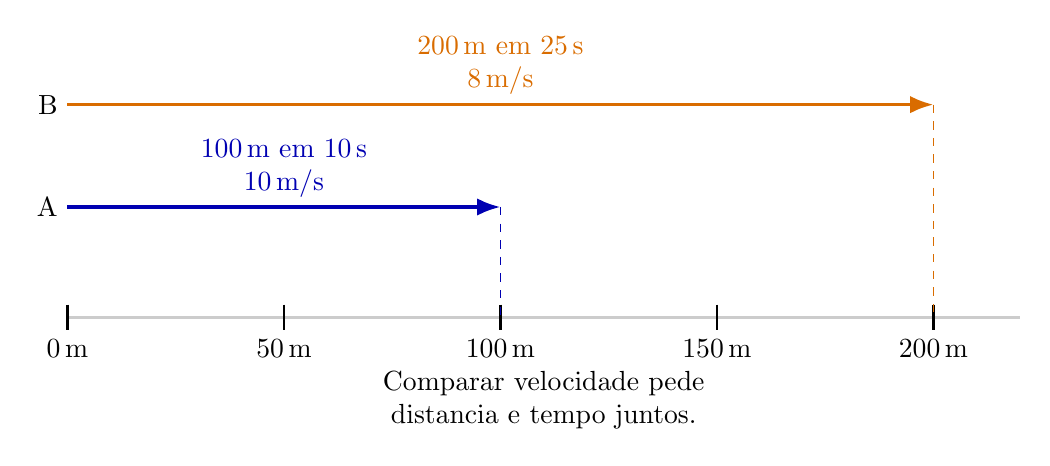
\begin{tikzpicture}[x=0.055cm,y=1cm,>=Latex]
  \draw[very thick,gray!40] (0,0) -- (220,0);
  \foreach \x in {0,50,100,150,200}{
    \draw[thick] (\x,0.16) -- (\x,-0.16);
    \node[below] at (\x,-0.16) {$\x\,\mathrm{m}$};
  }

  \draw[very thick,blue!70!black,->] (0,1.4) -- (100,1.4);
  \draw[very thick,orange!85!black,->] (0,2.7) -- (200,2.7);

  \node[left] at (0,1.4) {A};
  \node[left] at (0,2.7) {B};
  \node[above,align=center,blue!70!black] at (50,1.4) {$100\,\mathrm{m}$ em $10\,\mathrm{s}$\\$10\,\mathrm{m/s}$};
  \node[above,align=center,orange!85!black] at (100,2.7) {$200\,\mathrm{m}$ em $25\,\mathrm{s}$\\$8\,\mathrm{m/s}$};

  \draw[dashed,blue!70!black] (100,1.4) -- (100,0);
  \draw[dashed,orange!85!black] (200,2.7) -- (200,0);
  \node[align=center] at (110,-1.05) {Comparar velocidade pede\\distancia e tempo juntos.};
\end{tikzpicture}

% TikZ 2
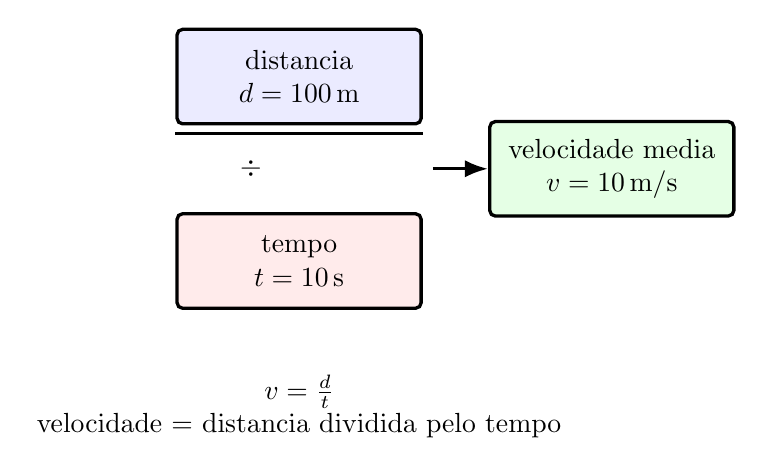
\begin{tikzpicture}[>=Latex,node distance=1.1cm]
  \tikzstyle{box}=[draw,rounded corners=2pt,minimum width=3.1cm,minimum height=1.2cm,align=center,very thick]
  \node[box,fill=blue!8] (d) {distancia\\$d=100\,\mathrm{m}$};
  \node[box,fill=red!8,below=of d] (t) {tempo\\$t=10\,\mathrm{s}$};
  \node[box,fill=green!10,right=2.4cm of $(d)!0.5!(t)$] (v) {velocidade media\\$v=10\,\mathrm{m/s}$};

  \draw[very thick] ($(d.south west)+(0,-0.1)$) -- ($(d.south east)+(0,-0.1)$);
  \node[left=0.35cm of $(d)!0.5!(t)$] {$\div$};
  \draw[very thick,->] ($(d)!0.5!(t)+(1.7,0)$) -- (v.west);

  \node[align=center,below=0.7cm of t] {$v=\frac{d}{t}$\\velocidade = distancia dividida pelo tempo};
\end{tikzpicture}

\end{document}
